\section{Horizontal scroll behaviour}
Skylines customers often have very large tables containing thousands of rows but also dozens of columns. Due to the large amount of columns that these tables contain, they often no longer fit into a single \gls{viewport}. To imitate reality as best as possible it should be possible to show a table larger than the width of the viewport. On a real website this would be done by adding a horizontal scroll bar.
    
\subsection{Adobe XD}
\subsection{Figma}
Supports horizontal scrolling behaviour
but does not show horizontal scrollbar. Which is not good for the user experience, since the user has no idea they can scroll to the right

No right click event support
\begin{figure}[h!]
\centering
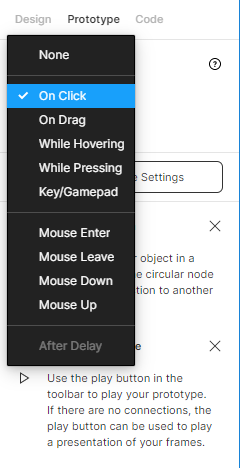
\includegraphics[scale=0.2]{figures/figma/figma-right-click-event.png}
\caption{Figma - Right Click Event}
\label{fig:figma-right-click-event}
\end{figure}

\subsection{Invision Studio}
Supports horizontal scrolling behaviour 
but does not show horizontal scroll bar. Which is not super ideal to test user experience, and that is where it's all about.

\subsection{Framer}